\documentclass[11pt, a4paper]{article}

\usepackage[margin=2.5cm]{geometry}
\usepackage{amsmath, amssymb}
\usepackage{booktabs}
\usepackage{graphicx}
\usepackage{hyperref}
\usepackage{microtype}
\usepackage{parskip}
\usepackage{xcolor}
\usepackage[round, sort&compress]{natbib}

\graphicspath{{figures/}}

% Placeholder macro – remove before submission
\newcommand{\TODO}[1]{\textcolor{red}{\textbf{[TODO: #1]}}}

\title{\textbf{Simulation-Based Inference for an Adaptive-Network SIR Model}}
\author{%
  \TODO{Florian Tobias Dreyer (A0338032M)} \and
  \TODO{Group member 2 (Student ID)} \and
  \TODO{Group member 3 (Student ID)}
}
\date{}

\begin{document}

\maketitle
\thispagestyle{empty}

% ============================================================
\section{Introduction}
\label{sec:intro}
% ============================================================

\TODO{Model motivation, data description, why likelihood is intractable.
Suggested length: $\sim$1 page.}

% ============================================================
\section{Model and Data}
\label{sec:model}
% ============================================================

\TODO{Formal model description: Erdős–Rényi network ($N=200$, $p=0.05$,
5 initially infected), three synchronous operations (Infection, Recovery,
Rewiring), and why the adaptive rewiring makes the likelihood intractable.
Reference \citet{gross2006}. Suggested length: $\sim$0.5 pages.}

The three unknown parameters have independent uniform priors:
$\beta \sim \mathcal{U}(0.05, 0.50)$,
$\gamma \sim \mathcal{U}(0.02, 0.20)$,
$\rho \sim \mathcal{U}(0.0, 0.8)$,
with prior standard deviations
$\sigma_\beta^{\mathrm{prior}} = 0.130$,
$\sigma_\gamma^{\mathrm{prior}} = 0.052$,
$\sigma_\rho^{\mathrm{prior}} = 0.231$.
The observed dataset comprises $R=40$ independent replicates, each providing
an infection time series, a rewiring time series, and a final degree distribution
(Figure~\ref{fig:obs_data}).

\begin{figure}[h]
  \centering
  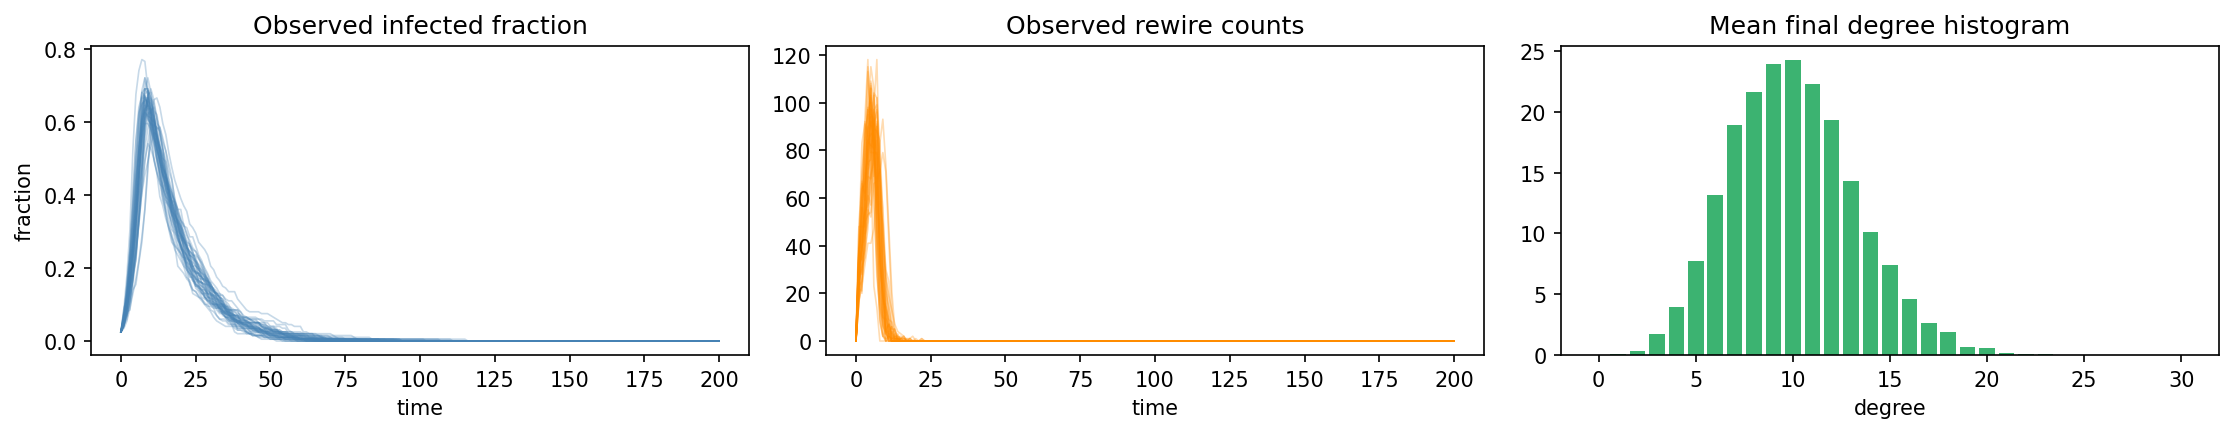
\includegraphics[width=\textwidth]{obs_data}
  \caption{Observed data across 40 replicates: infection fraction (left),
           rewiring events (centre), final degree distribution (right).}
  \label{fig:obs_data}
\end{figure}

% ============================================================
\section{Summary Statistics}
\label{sec:summaries}
% ============================================================

Because acceptance probability in ABC falls exponentially with summary
dimension \citep{blum2013}, we compress the raw time series to a
15-dimensional \emph{balanced} feature vector averaged across replicates:
five infection summaries (peak fraction, epidemic duration, total infection,
and their cross-replicate standard deviations),
four rewiring summaries (total events, peak rate, and standard deviations), and
six degree summaries (mean, std, entropy, quartiles of the final degree
distribution).

\subsection{Identifiability diagnostics}

Projecting the $M=10\,000$ prior-simulation summaries to 2D via PCA and
colouring by parameter value (Figure~\ref{fig:pca}) reveals clear gradients
for $\gamma$, moderate structure for $\beta$, and weak but non-trivial
structure for $\rho$.
This confirms the central identifiability challenge: $\beta$ and $\rho$
both suppress the epidemic — via higher transmission rate being countered by
faster recovery ($\gamma$) or network rewiring ($\rho$) — so infection-curve
summaries alone cannot fully separate them. Rewiring summaries carry
independent information about both $\beta$ and $\rho$.

\begin{figure}[h]
  \centering
  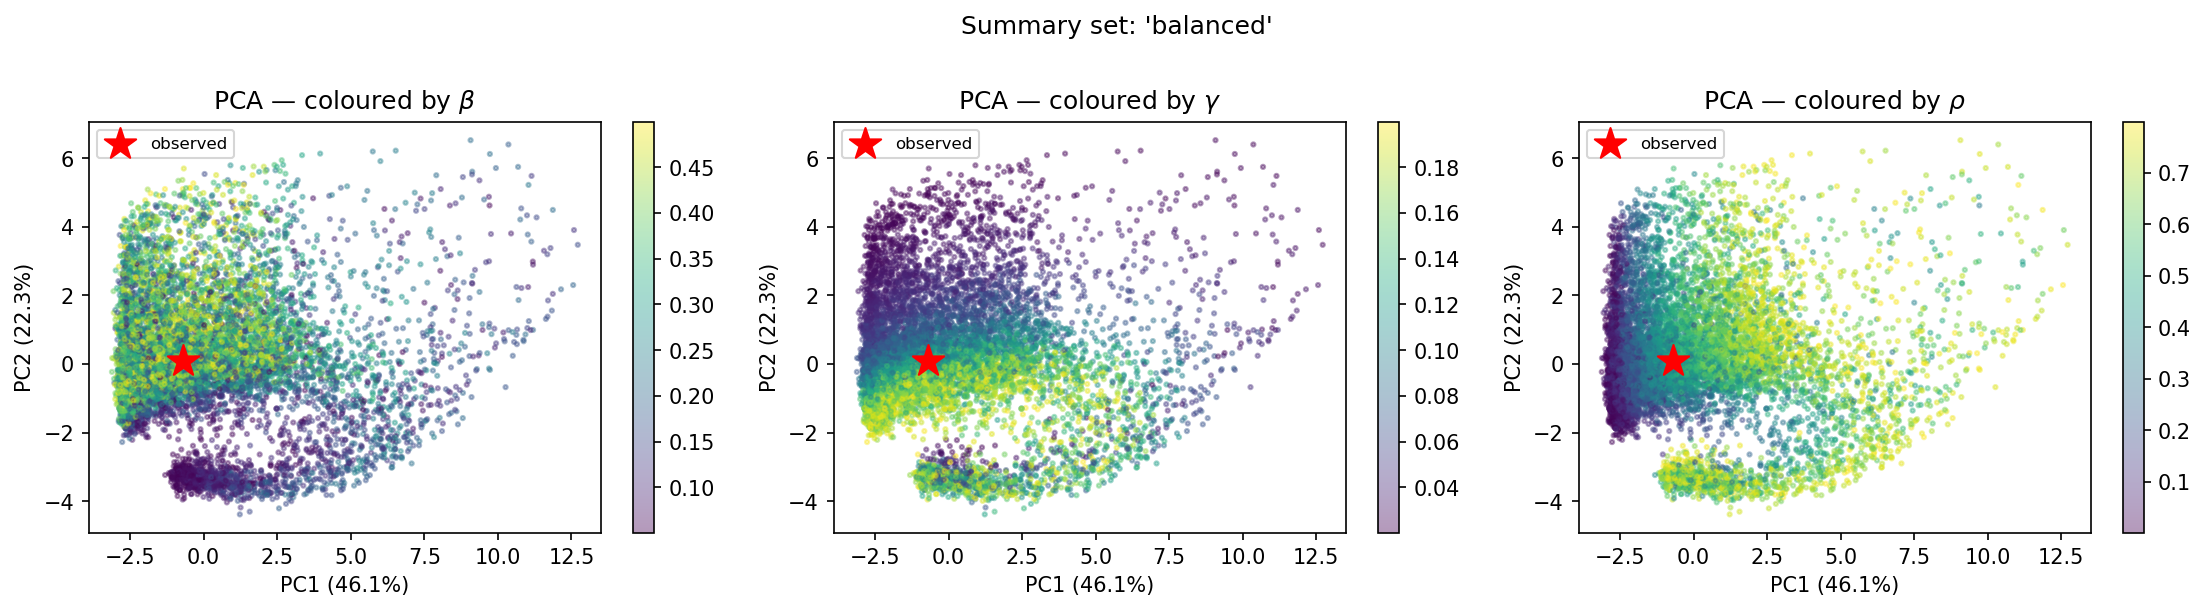
\includegraphics[width=\textwidth]{pca_diagnostic}
  \caption{PCA diagnostic: prior simulations coloured by $\beta$, $\gamma$,
           $\rho$ (left to right). Clear gradients for $\gamma$; partial
           confounding visible in $\beta$–$\rho$ panels.}
  \label{fig:pca}
\end{figure}

\subsection{Summary-set comparison}

We evaluated four candidate sets at $q=1\%$.
Table~\ref{tab:sumset} and Figure~\ref{fig:sumset_heatmap} report posterior
std relative to prior std (lower = more informative).

\begin{table}[h]
\centering
\caption{Relative posterior std (std\,/\,prior std) per summary set at $q=1\%$.
         Bold marks the best set for each parameter.}
\label{tab:sumset}
\begin{tabular}{lrrr}
\toprule
Set & $\beta$ & $\gamma$ & $\rho$ \\
\midrule
infection\_only & 0.377 & \textbf{0.084} & 0.854 \\
rewiring\_only  & \textbf{0.216} & 0.804 & \textbf{0.173} \\
degree\_only    & 0.924 & 0.932 & 0.483 \\
balanced        & 0.479 & 0.378 & 0.262 \\
\bottomrule
\end{tabular}
\end{table}

The results reveal a clear separation of information sources:
$\gamma$ is almost entirely encoded in the infection curve
(\textit{infection\_only} reduces its posterior to 8\% of the prior width),
while both $\beta$ and $\rho$ are best identified from rewiring summaries
(\textit{rewiring\_only} achieves relative widths of 0.22 and 0.17
respectively).
The degree distribution alone carries little information about $\beta$ or
$\gamma$, but provides moderate constraint on $\rho$ (0.48).

No single-source set identifies all three parameters well simultaneously.
The \emph{balanced} set is a deliberate compromise: it sacrifices some
per-parameter sharpness in exchange for robustness across all three, and
is used in all subsequent analyses.

\begin{figure}[h]
  \centering
  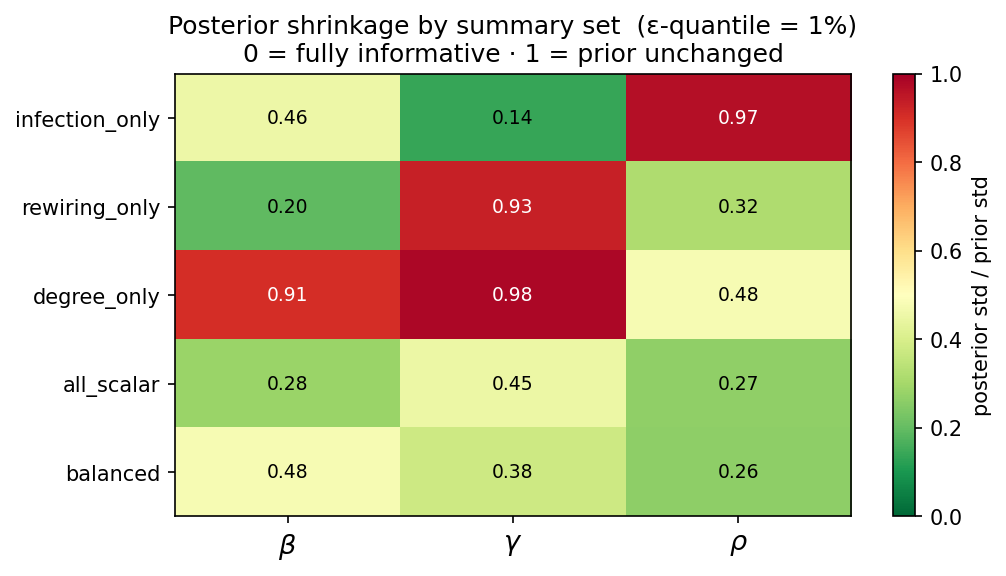
\includegraphics[width=0.7\textwidth]{sumset_heatmap}
  \caption{Posterior std (relative to prior) per summary set and parameter
           at $q=1\%$. Lower is more informative.}
  \label{fig:sumset_heatmap}
\end{figure}

% ============================================================
\section{Rejection ABC}
\label{sec:rabc}
% ============================================================

We drew $M=10\,000$ prior samples, computed the standardised Euclidean distance
between each simulated and observed summary vector, and accepted draws below the
1\% empirical quantile \citep{pritchard1999}, giving $\varepsilon=1.2852$ and
$n_\mathrm{acc}=100$.
Figure~\ref{fig:rabc_posteriors} shows the marginal posteriors; Table~\ref{tab:rabc}
gives the numerical summaries.

\begin{figure}[h]
  \centering
  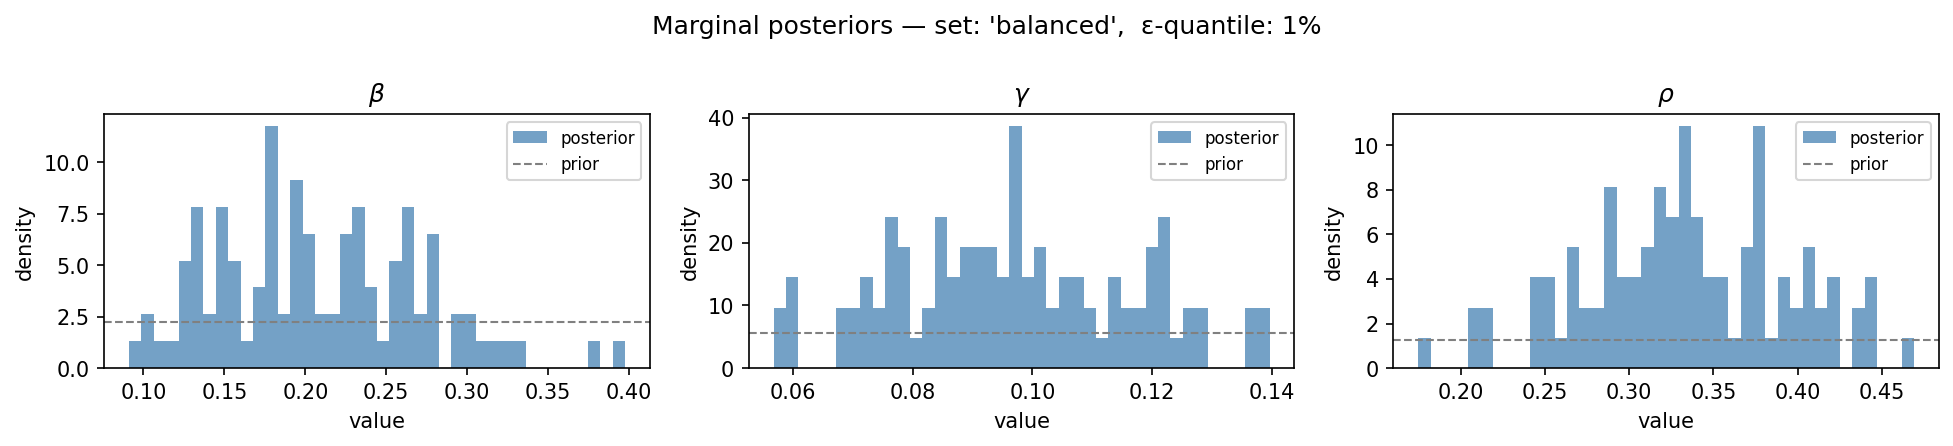
\includegraphics[width=\textwidth]{rabc_marginals}
  \caption{Rejection ABC marginal posteriors (blue) vs.\ uniform prior (dashed),
           \emph{balanced} set, $\varepsilon=1.2852$, $n_\mathrm{acc}=100$.}
  \label{fig:rabc_posteriors}
\end{figure}

\begin{table}[h]
\centering
\caption{Rejection ABC posterior ($q=1\%$, \emph{balanced}).}
\label{tab:rabc}
\begin{tabular}{lrrrrr}
\toprule
Param & Mean & Std & 25\% & Median & 75\% \\
\midrule
$\beta$  & 0.208 & 0.063 & 0.159 & 0.201 & 0.254 \\
$\gamma$ & 0.097 & 0.020 & 0.083 & 0.096 & 0.112 \\
$\rho$   & 0.334 & 0.061 & 0.291 & 0.332 & 0.378 \\
\bottomrule
\end{tabular}
\end{table}

$\gamma$ is best-identified (directly controls epidemic duration),
$\beta$ moderately so, and $\rho$ is hardest to constrain — consistent with
the PCA diagnostic and the negative $(\beta,\rho)$ posterior correlation
driven by their shared epidemic-suppression effect.

% ============================================================
\section{Advanced Methods}
\label{sec:advanced}
% ============================================================

\subsection{Semi-Automatic ABC \citep{fearnhead2012}}
\label{sec:semiauto}

\citet{fearnhead2012} show that the optimal ABC summaries are the
posterior means $\mathbb{E}[\theta\mid x]$, which can be approximated by
fitting Ridge regression from the balanced features to each parameter on
the pilot draws.
In-sample $R^2$ values confirm strong predictability:
$R^2_\beta=0.812$, $R^2_\gamma=0.857$, $R^2_\rho=0.979$.
Running rejection ABC in the resulting 3-dimensional projected space
($\varepsilon=0.520$, $n_\mathrm{acc}=100$) substantially tightens the
posterior for $\beta$ and provides moderate gains for $\gamma$ and $\rho$
(Figure~\ref{fig:semiauto}, Table~\ref{tab:contraction}).

\begin{figure}[h]
  \centering
  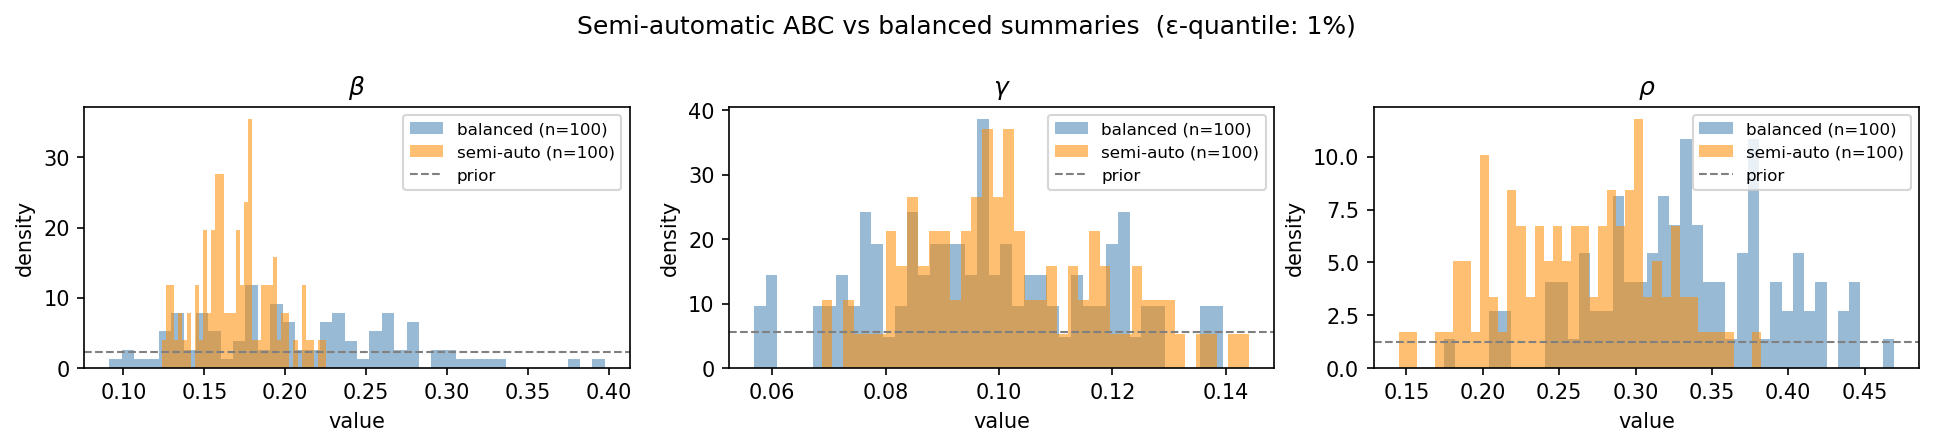
\includegraphics[width=\textwidth]{semiauto_marginals}
  \caption{Balanced rejection ABC (blue) vs.\ semi-automatic ABC (orange),
           $q=1\%$.}
  \label{fig:semiauto}
\end{figure}

\subsection{LASSO-Based Summary Selection \citep{blum2013}}
\label{sec:lasso}

Fitting LassoCV from summaries to each parameter on the pilot simulations
retained 14/15 features for $\beta$ ($\alpha=6\times10^{-4}$) and all 15 for
$\gamma$ and $\rho$ ($\alpha=8\times10^{-4}$).
No feature is entirely redundant, so the LASSO-selected set is
effectively identical to the balanced set and yields the same posterior
(Table~\ref{tab:contraction}).

\begin{table}[h]
\centering
\caption{Posterior std and relative contraction (std/prior std) for
         rejection ABC variants at $q=1\%$.}
\label{tab:contraction}
\begin{tabular}{lrrrrrr}
\toprule
& \multicolumn{2}{c}{$\beta$} & \multicolumn{2}{c}{$\gamma$} & \multicolumn{2}{c}{$\rho$} \\
\cmidrule(lr){2-3}\cmidrule(lr){4-5}\cmidrule(lr){6-7}
Method & Std & Rel. & Std & Rel. & Std & Rel. \\
\midrule
Prior          & 0.130 & 1.00 & 0.052 & 1.00 & 0.231 & 1.00 \\
Balanced (15d) & 0.062 & 0.48 & 0.020 & 0.38 & 0.061 & 0.26 \\
LASSO (15d)    & 0.062 & 0.48 & 0.020 & 0.38 & 0.061 & 0.26 \\
Semi-auto (3d) & 0.023 & 0.18 & 0.017 & 0.33 & 0.051 & 0.22 \\
\bottomrule
\end{tabular}
\end{table}

\subsection{Regression Adjustment \citep{beaumont2002}}
\label{sec:regadj}

After accepting draws at a loose tolerance ($q=5\%$, $\varepsilon=1.706$,
$n_\mathrm{acc}=500$), each accepted $\theta^{(i)}$ is corrected for the
residual gap between its simulated summary $s^{(i)}$ and $s_\mathrm{obs}$:
\[
  \tilde{\theta}^{(i)}
    = \theta^{(i)} - \hat{B}^\top (s^{(i)} - s_\mathrm{obs}),
\]
where $\hat{B}$ is estimated by weighted least squares with Epanechnikov
kernel weights \citep{beaumont2002}.
Figure~\ref{fig:regadj_marginals} and Table~\ref{tab:regadj} show that
adjustment dramatically sharpens the posterior
($\sigma_\beta$: 0.099$\to$0.024, $\sigma_\gamma$: 0.033$\to$0.007,
$\sigma_\rho$: 0.087$\to$0.008).
Crucially, the adjusted posterior is nearly tolerance-invariant for
$q\lesssim10\%$ (Figure~\ref{fig:regadj_width}), whereas the raw posterior
degrades rapidly at loose tolerances.

\begin{figure}[h]
  \centering
  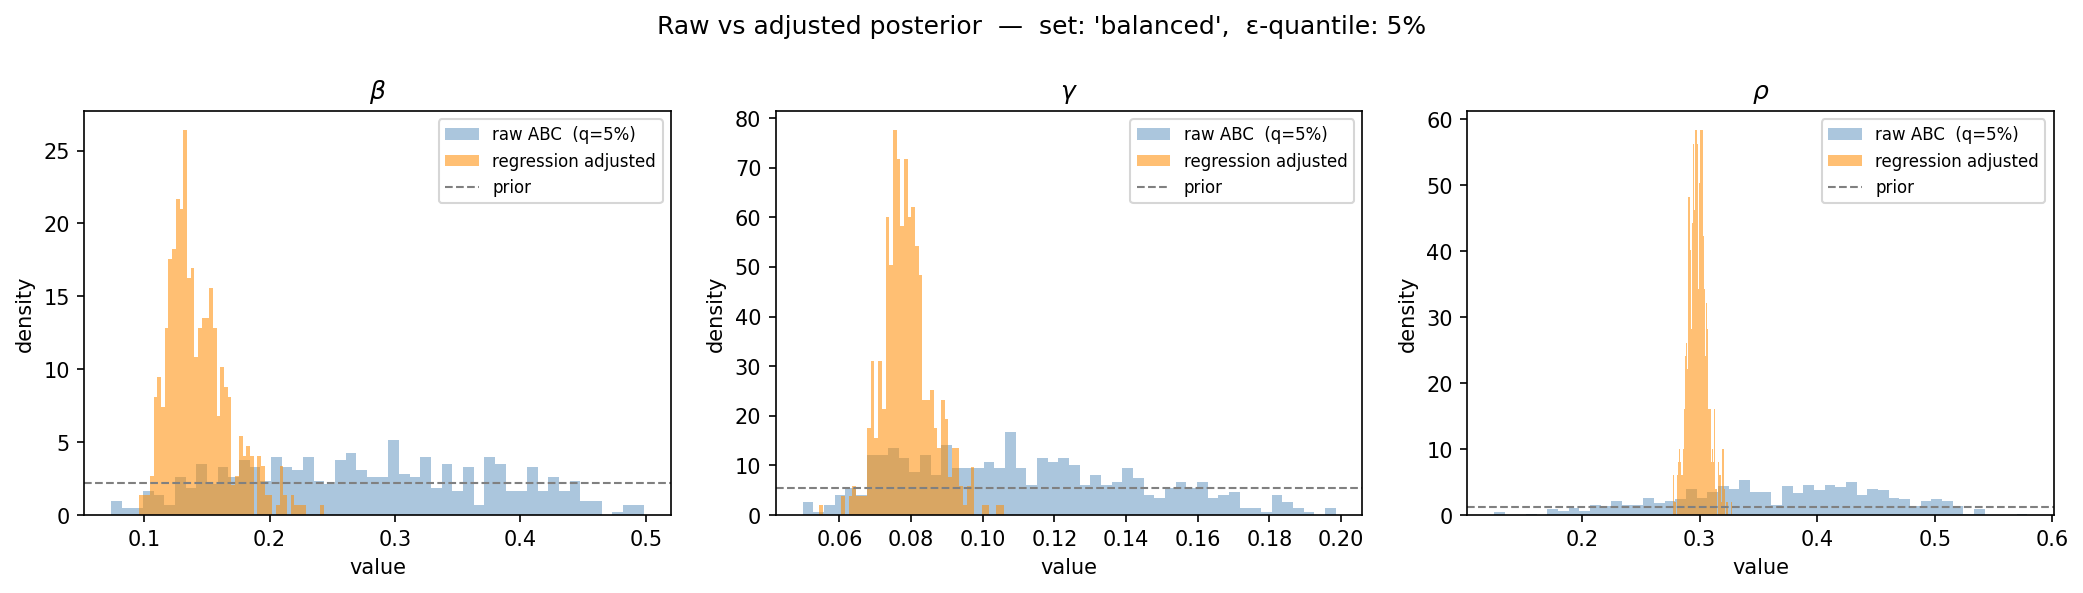
\includegraphics[width=\textwidth]{regadj_marginals}
  \caption{Raw ABC (blue) vs.\ regression-adjusted (orange) posteriors,
           $q=5\%$, \emph{balanced} set.}
  \label{fig:regadj_marginals}
\end{figure}

\begin{table}[h]
\centering
\caption{Raw vs.\ regression-adjusted posteriors ($q=5\%$).}
\label{tab:regadj}
\begin{tabular}{llrrrrr}
\toprule
Method & Param & Mean & Std & 5\% & Median & 95\% \\
\midrule
Raw ($q=5\%$) & $\beta$  & 0.276 & 0.099 & 0.127 & 0.272 & 0.439 \\
              & $\gamma$ & 0.111 & 0.033 & 0.066 & 0.108 & 0.169 \\
              & $\rho$   & 0.367 & 0.087 & 0.216 & 0.373 & 0.504 \\
\addlinespace
Adjusted      & $\beta$  & 0.143 & 0.024 & 0.112 & 0.138 & 0.191 \\
              & $\gamma$ & 0.079 & 0.007 & 0.069 & 0.078 & 0.092 \\
              & $\rho$   & 0.299 & 0.008 & 0.286 & 0.298 & 0.313 \\
\bottomrule
\end{tabular}
\end{table}

\begin{figure}[h]
  \centering
  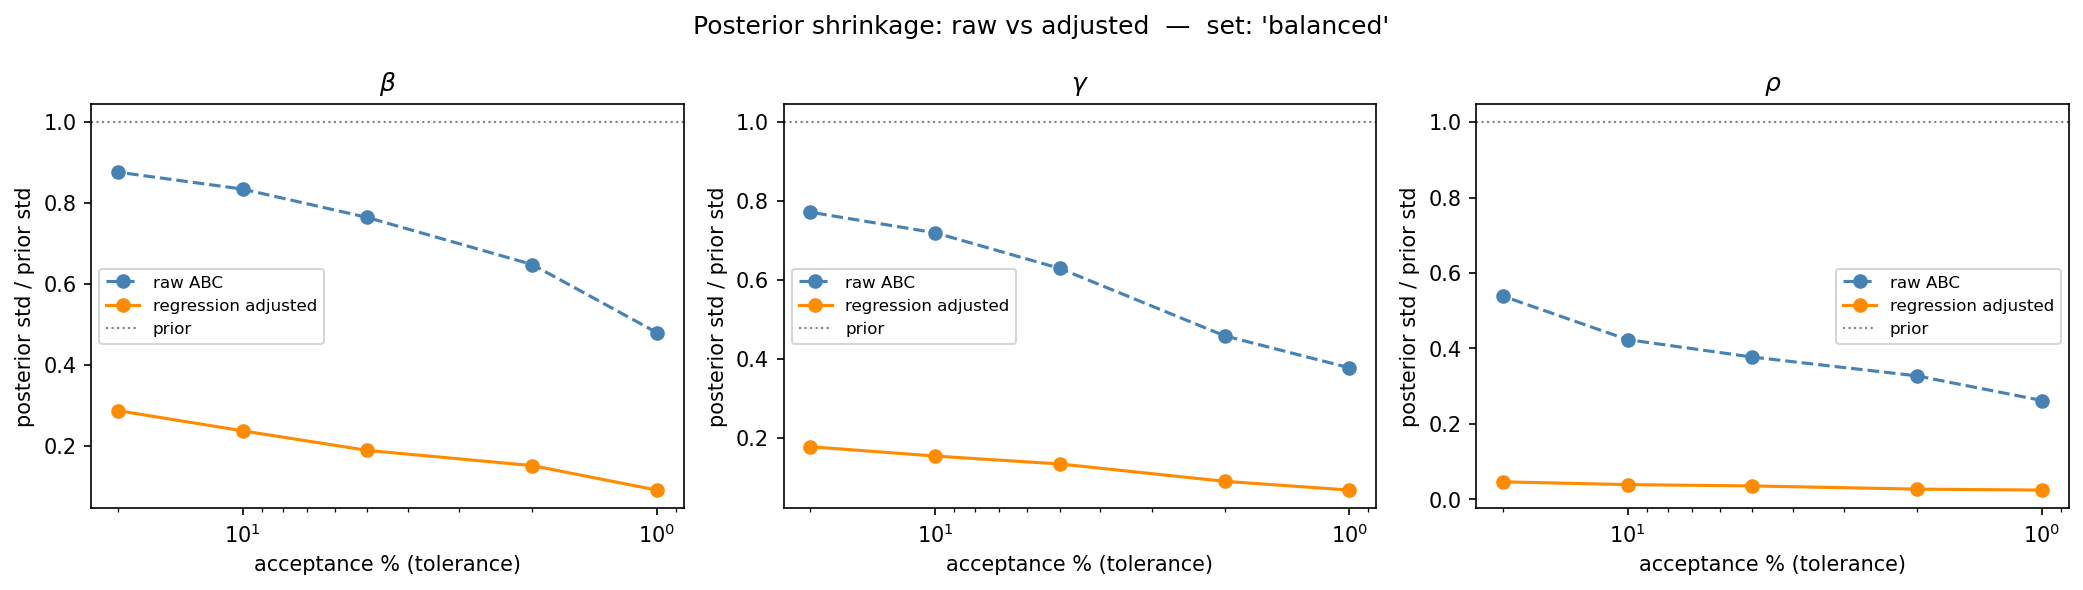
\includegraphics[width=\textwidth]{regadj_width}
  \caption{Posterior std (relative to prior) vs.\ tolerance $q$ for raw (blue)
           and adjusted (orange) ABC. Adjustment is approximately
           tolerance-invariant for $q\lesssim10\%$.}
  \label{fig:regadj_width}
\end{figure}

\subsection{Synthetic Likelihood \citep{wood2010}}
\label{sec:sl}

At each MCMC proposal $\theta$, we simulate $N_\mathrm{sim}=50$ datasets
($R_\mathrm{sim}=40$ replicates each) and approximate the intractable
likelihood as a multivariate Gaussian fitted to the $N_\mathrm{sim}$ summary
vectors, using Ledoit--Wolf shrinkage for the covariance
\citep{ledoitwolf2004}:
\[
  \log\hat{p}_\mathrm{SL}(s_\mathrm{obs}\mid\theta)
  = \log\mathcal{N}(s_\mathrm{obs};\,\hat{\mu}(\theta),\,\hat{\Sigma}(\theta)).
\]
This is embedded in a Metropolis--Hastings random-walk MCMC
($N_\mathrm{steps}=2\,000$, burn-in $=500$, step sizes
$\sigma=(0.04, 0.015, 0.06)$).

The acceptance rate was $\approx1$–$3\%$ (target: 20–40\%), resulting in
very low effective sample sizes ($\mathrm{ESS}\approx4$–$5$ from 1\,501
post-burn-in samples), as visible in the trace and autocorrelation plots
(Figure~\ref{fig:sl_trace}).
Despite poor mixing, the chain clusters consistently around
$(\hat\beta,\hat\gamma,\hat\rho)\approx(0.152, 0.080, 0.302)$, in agreement
with the regression-adjusted medians.
The reported posterior standard deviations (Table~\ref{tab:sl}) are therefore
underestimates of the true posterior width.
Remedies include reducing step sizes, using an adaptive proposal, or switching
to a gradient-based sampler.

\begin{figure}[h]
  \centering
  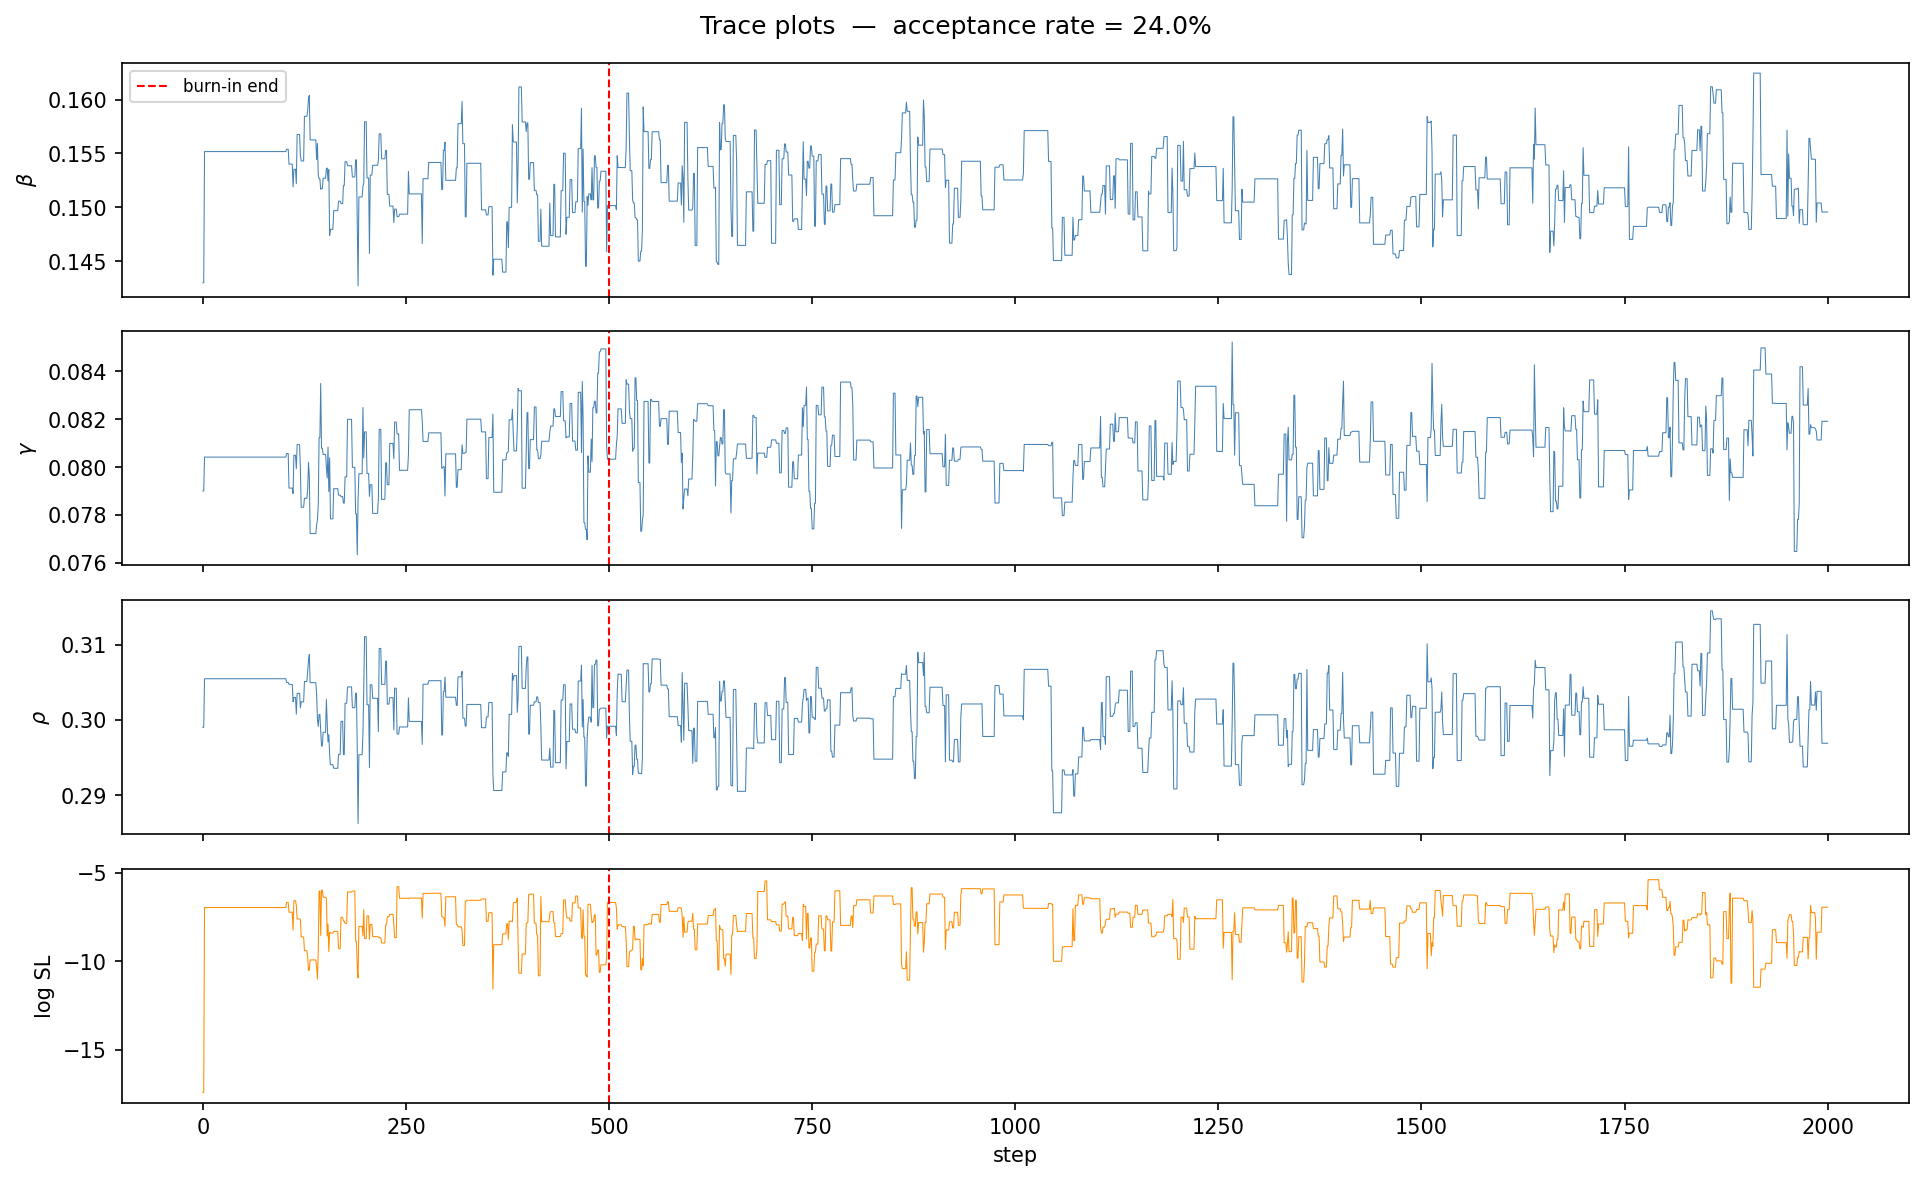
\includegraphics[width=\textwidth]{sl_trace}
  \caption{MCMC trace plots. The chain shows prolonged stagnation, reflecting
           the low acceptance rate. Autocorrelation remains near 1.0 throughout,
           confirming ESS $\approx4$–$5$.}
  \label{fig:sl_trace}
\end{figure}

\begin{figure}[h]
  \centering
  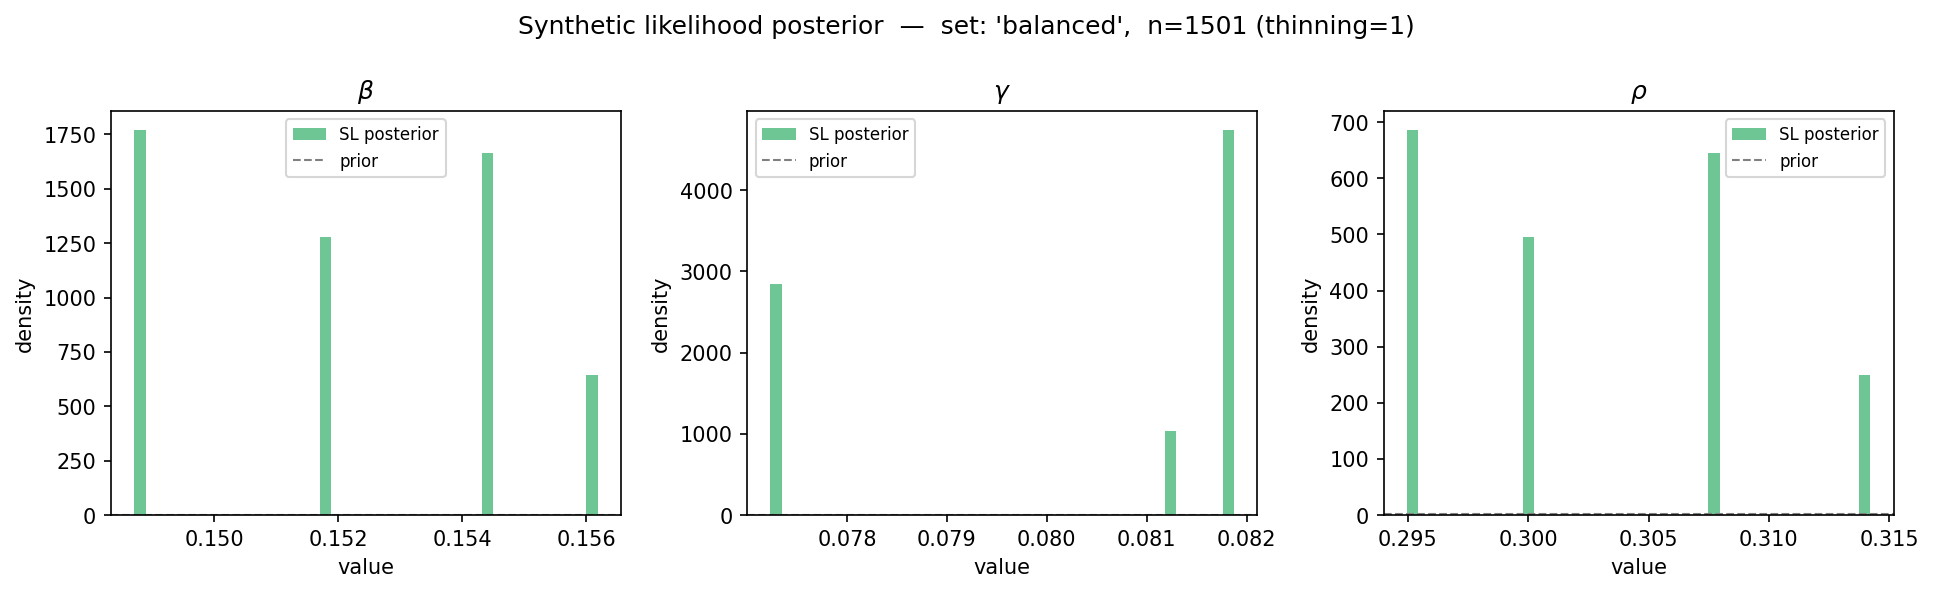
\includegraphics[width=\textwidth]{sl_marginals}
  \caption{Synthetic likelihood MCMC posterior (green) vs.\ prior (dashed).
           Narrow widths reflect chain stagnation rather than true posterior
           precision.}
  \label{fig:sl_marginals}
\end{figure}

\begin{table}[h]
\centering
\caption{Synthetic likelihood MCMC posterior (1\,501 post-burn-in samples).
         Low ESS: std values are lower bounds on true posterior width.}
\label{tab:sl}
\begin{tabular}{lrrrrrr}
\toprule
Param & Mean & Std & 5\% & Median & 95\% & ESS \\
\midrule
$\beta$  & 0.152 & 0.003 & 0.149 & 0.152 & 0.156 & 4 \\
$\gamma$ & 0.080 & 0.002 & 0.077 & 0.082 & 0.082 & 5 \\
$\rho$   & 0.302 & 0.007 & 0.295 & 0.300 & 0.314 & 4 \\
\bottomrule
\end{tabular}
\end{table}

% ============================================================
\section{Comparison}
\label{sec:comparison}
% ============================================================

Table~\ref{tab:compare} summarises all methods.
Point estimates are consistent across advanced methods
($\hat\beta\approx0.14$–$0.21$, $\hat\gamma\approx0.08$–$0.11$,
$\hat\rho\approx0.30$).
Regression adjustment gives the most reliable uncertainty quantification:
large accepted set ($n=500$), tolerance-robust, and verifiable via
sensitivity analysis.
The SL chain provides a useful point estimate but requires better
step-size tuning before its uncertainty intervals can be trusted.

\begin{table}[h]
\centering
\caption{Posterior standard deviations across all methods.
         $^\dagger$SL chain not converged; std values are lower bounds.}
\label{tab:compare}
\begin{tabular}{lrrrr}
\toprule
Method & $\sigma_\beta$ & $\sigma_\gamma$ & $\sigma_\rho$ & Notes \\
\midrule
Prior                  & 0.130 & 0.052 & 0.231 & -- \\
Rej.\ ABC ($q=1\%$)    & 0.062 & 0.020 & 0.061 & $n=100$ \\
LASSO ($q=1\%$)        & 0.062 & 0.020 & 0.061 & All 15 features kept \\
Semi-auto ($q=1\%$)    & 0.023 & 0.017 & 0.051 & 3-d projection \\
Reg.\ adj.\ ($q=5\%$)  & 0.024 & 0.007 & 0.008 & $n=500$, robust \\
Synth.\ lik.$^\dagger$ & 0.003 & 0.002 & 0.007 & ESS~$\approx4$ \\
\bottomrule
\end{tabular}
\end{table}

\TODO{If additional methods (ABC-MCMC, SMC-ABC) were implemented, add a
subsection here.}

% ============================================================
\section{Conclusion}
\label{sec:conclusion}
% ============================================================

\TODO{Summarise: (1) identifiability findings; (2) how each method improves
on basic rejection ABC; (3) SL mixing limitations and future work.
Suggested length: $\sim$0.5 pages.}

% ============================================================
\bibliographystyle{plainnat}
\bibliography{references}

\end{document}
